\chapter{Introdução} \label{ch:intro}

	O ensino de Engenharia no Brasil se inicia formalmente em 1792, com a criação da Real Academia de Artilharia, Fortificação e Desenho, na cidade do Rio de Janeiro. Esta foi precursora da Escola Politécnica da Universidade Federal do Rio de Janeiro (Poli\abbrev{Poli}{Escola Politécnica}/UFRJ\abbrev{UFRJ}{Universidade Federal do Rio de Janeiro}) e também do Instituto Militar de Engenharia.\\
	
	%Apesar desta instituição ter sido pioneira na América Latina, o Brasil hoje apresenta uma proporção de engenheiros formados relativamente baixa em relação ao total de profissionais egressos das Instituições de Ensino Superior, quando comparado com outros países índice de desenvolvimento humano semelhante \cite{evolucao-formacao-engenheiros-ipea}.\\
	
	A regulamentação nacional da profissão de Engenheiro se dá em 1933, com a criação do Conselho Federal de Engenharia e Arquitetura e dos respectivos Conselhos Regionais, em resposta ao surgimento de outras unidades de ensino através do país e da necessidade de proteger o mercado de profissionais leigos ou inabilitados \cite{historia-confea}.\\
	
	Nas últimas décadas o número de instituições de ensino e de cursos de engenharia reconhecidos pelo Ministério da Educação vêm apresentando crescimento quantitativo notável, conforme evidenciado pela figura \ref{fig:evolucaocursosengenharias}, que mostra a evolução na quantidade de cursos de engenharia elétrica, eletrônica e afins em Instituições de Ensino Superior (IES\abbrev{IES}{Instituição de Ensino Superior}) públicas e privadas.\\
	
	\begin{figure}[h!]
		\centering
		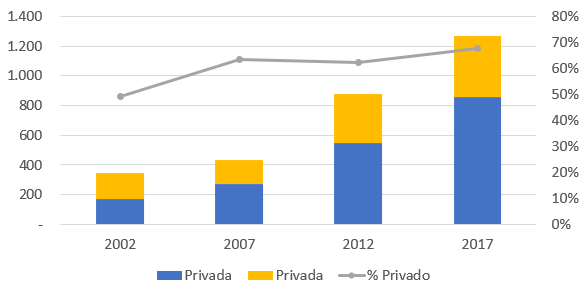
\includegraphics[width=0.75\linewidth]{Figuras/evolucao_cursos_engenharias}
		\caption[Evolução da quantidade de cursos de engenharia elétrica, eletrônica e afins]{Evolução da quantidade de cursos de engenharia elétrica, eletrônica e afins e a respectiva relação entre instituições públicas e privadas}
		\label{fig:evolucaocursosengenharias}
	\end{figure}
	
	

	\section{Motivação}

		A produção de ciência e tecnologia é cada vez mais relevante não só para o desenvolvimento socioeconômico, mas para a soberania nacional como um todo. Neste contexto, é bastante estratégico que seja feita uma reflexão sobre o modelo adotado para construção de conhecimento necessário à formação das próximas gerações de engenheiros.\\
		
		Esta análise se torna ainda mais importante quando se considerando a realidade das IES públicas, já que estas seriam polos para produção de conhecimento voltado para o transformação das sociedades em que se inserem.\\
		
		A figura \ref{fig:evolucaomatriculadosconcluintes} mostra e evolução do volume de estudantes matriculados em cursos de engenharia elétrica, eletrônica e afins e a razão entre a quantidade de concluintes e total de matriculados, considerando IES públicas e privadas.
		
		\begin{figure}[h!]
			\centering
			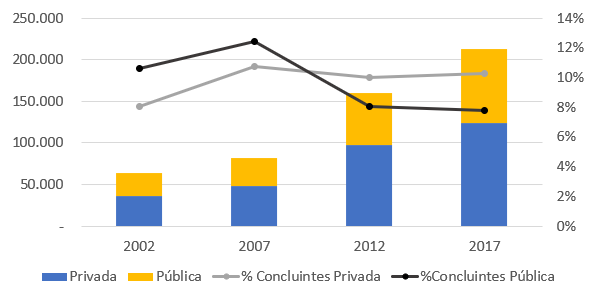
\includegraphics[width=0.75\linewidth]{Figuras/evolucao_matriculados_concluintes}
			\caption[Evolução de matriculados em cursos de engenharia elétrica, eletrônica e afins]{Evolução da quantidade de estudantes matriculados em cursos de engenharia elétrica, eletrônica e afins e a proporção de concluintes sobre o total, em instituições públicas e privadas}
			\label{fig:evolucaomatriculadosconcluintes}
		\end{figure}
		
		
		
	\section{Objetivos}
	
		Este trabalho faz a análise das possibilidades de implementação da metodologia de \textit{Problem Based Learning} no curso de Engenharia Elétrica da Poli/UFRJ.
		
	\section{Estrutura}
	
		Este trabalho está dividido em 5 capítulos:\\
		
		O \textbf{Capítulo \ref{ch:revisao}} apresenta uma revisão bibliográfica d
		
		O \textbf{Capítulo \ref{ch:metodo}} mostra o método aplicado na proposta de implementação da metodologia.
		
		O \textbf{Capítulo \ref{ch:resultados}} faz uma análise dos resultados esperados 
		
		O \textbf{Capítulo \ref{ch:conclusoes}} apresenta as conclusões e as propostas de projetos futuros.